\documentclass[cn,pad,chinese,chinesefont=nofont,math=newtx]{elegantbook}
\usepackage{latexgit}
\usepackage{hyperref}
\hypersetup{
	pdftitle={洞箫演奏 - 筒音5},
    pdfauthor={雪散舞}
}
%\usepackage{showframe}
\setCJKmainfont{Source Han Serif} 
\setCJKsansfont{Source Han Sans} 
\setCJKmonofont{Source Han Mono} 
\setCJKfamilyfont{zhsong}{Source Han Serif}
\setCJKfamilyfont{zhhei}{Source Han Sans} 
\setCJKfamilyfont{zhkai}{Source Han Mono} 
\setCJKfamilyfont{zhfs}{Source Han Mono} 
\newcommand*{\songti}{\CJKfamily{zhsong}} 
\newcommand*{\heiti}{\CJKfamily{zhhei}} 
\newcommand*{\kaishu}{\CJKfamily{zhkai}} 
\newcommand*{\fangsong}{\CJKfamily{zhfs}}

\title{洞箫集谱}
\author{雪散舞}
\date{\zhtoday}
\cover{dongxiao/cover.jpeg}
\logo{monk.png}
\extrainfo{清籁远喑喑,秦楼夜思深。碧空人已去,沧海凤难寻。\\杳妙和云绝,依微向水沉。还将九成意,高阁伫芳音。}
\version{\gitcommithash}

\begin{document}
\maketitle
\frontmatter
\tableofcontents
\mainmatter

\chapter{箫的来历}
\paragraph*{箫,形声。字从竹从肃,肃亦声。“肃”本义为“千针万孔”,转义为“风声尖锐地漫天呼啸”。“竹”与“肃”联合起来表示“一种模拟风声漫天尖锐呼啸的竹制吹奏乐器”。本义:一种模拟风吹声的竹乐器。}
\paragraph*{箫源于远古时期的骨哨,历史上亦称为笛,唐以后方专指竖吹之笛。“横吹笛子竖吹箫”,即笛箫之间最基本的差别。箫历史悠久,音色圆润轻柔,幽静典雅,适于独奏和重奏。箫笛同源于远古时期的骨哨,新石器时代开始以竹制作。在秦汉至唐,箫是指编管的排箫。} 
\paragraph*{早在《尚书·益稷》中记载有“箫韶九成,凤凰来仪。”当因韶乐伴奏乐器以箫(当时为排箫)为主而有此称。箫在汉代时称为“篴”、“竖篴”。西晋乐工列和、中书监荀勖所改革的笛为6 孔(前5、后1),其形制与今天的箫已非常相似了。东晋的桓伊,擅长音乐,他有一支蔡邕的柯亭笛(箫),是江南数第一的吹箫名手,地位和声望都已很高。他曾为素不相识的王徽之吹奏过三段乐曲,在历史上被传为佳话。}
\paragraph*{魏晋南北朝时,箫已用于独奏、合奏,并在伴奏相和歌的乐队中使用。清代,箫的形制完全一样。清《律吕正义后编》记载:“明时乃直曰箫,不复有竖篴。今箫长一尺八寸弱,从上口吹,有后出孔;笛横吹,无后出孔。”}

\chapter{八孔箫指法图}
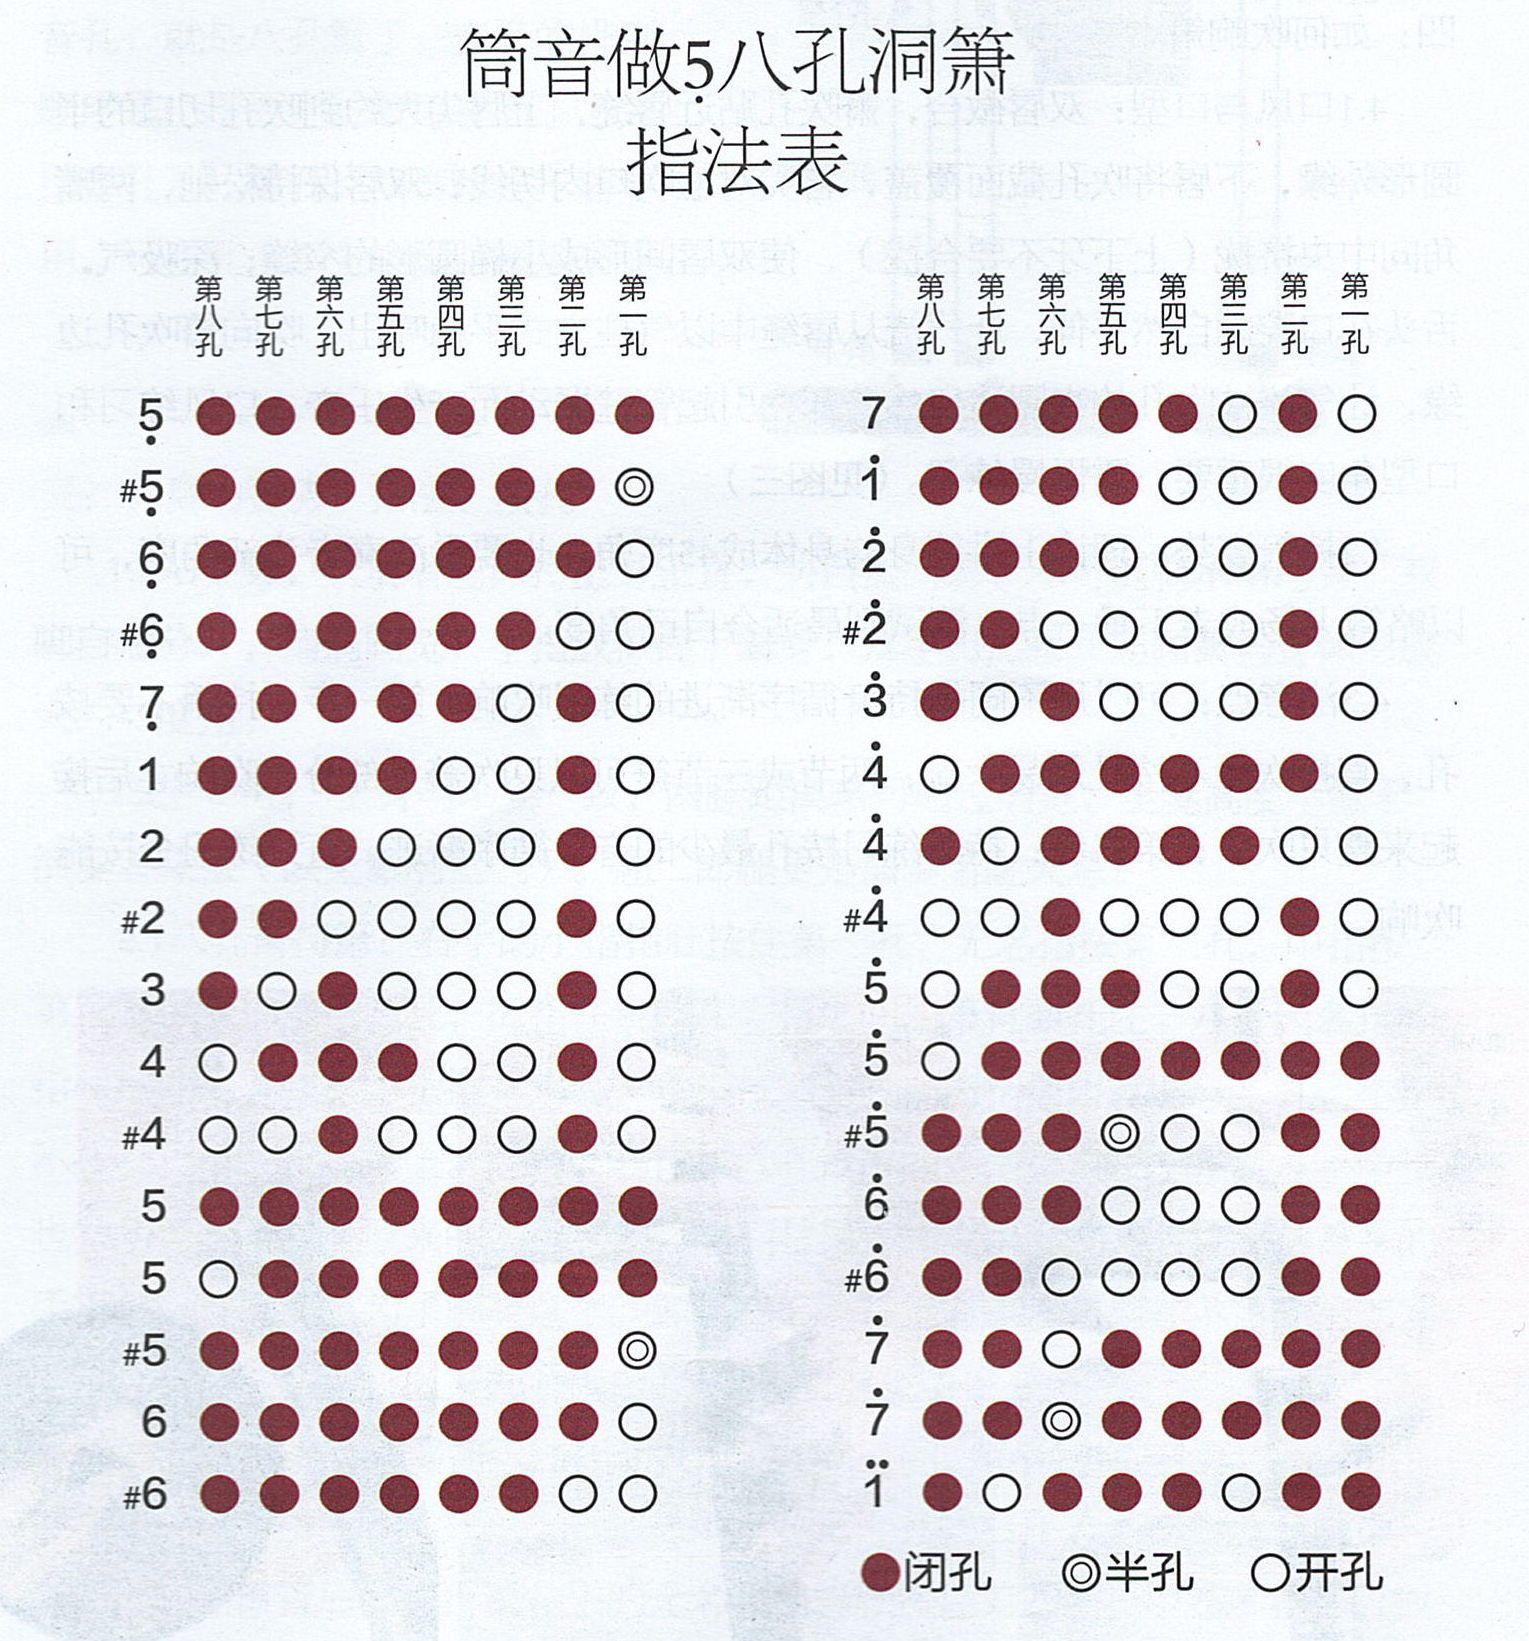
\includegraphics[width=0.93\textwidth]{dongxiao/Scan.jpeg}
\chapter{练习谱 - 筒音作5}
\begin{center}
	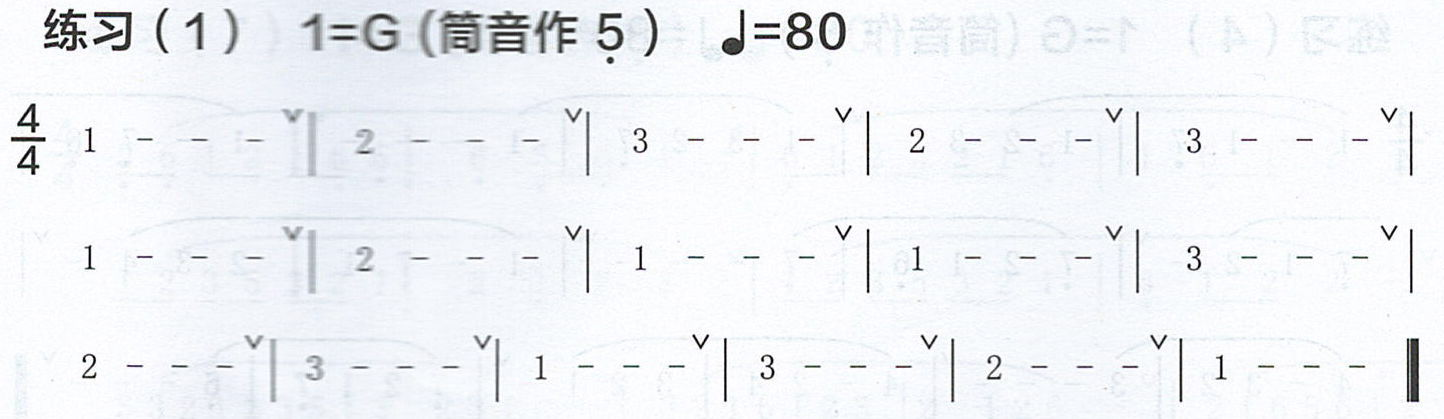
\includegraphics[width=\textwidth]{dongxiao/Scan 1-1.jpeg}
	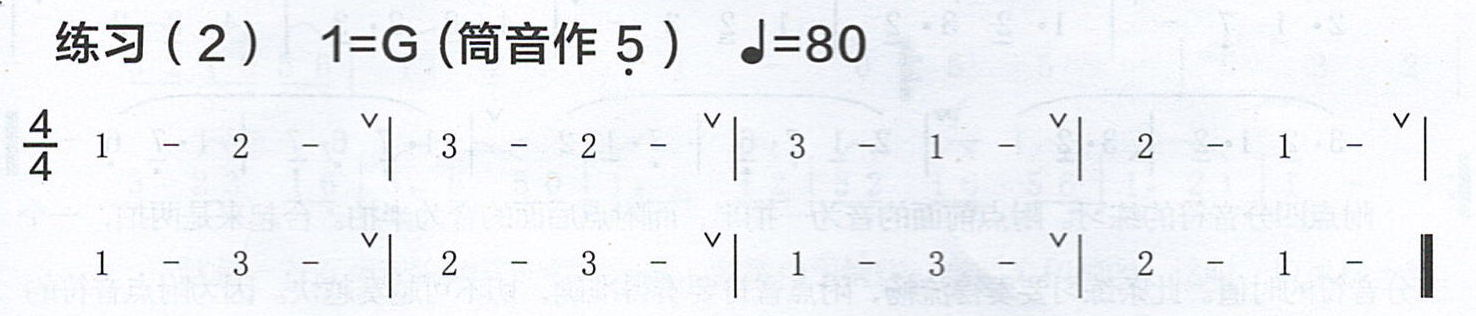
\includegraphics[width=\textwidth]{dongxiao/Scan 1-2.jpeg}
	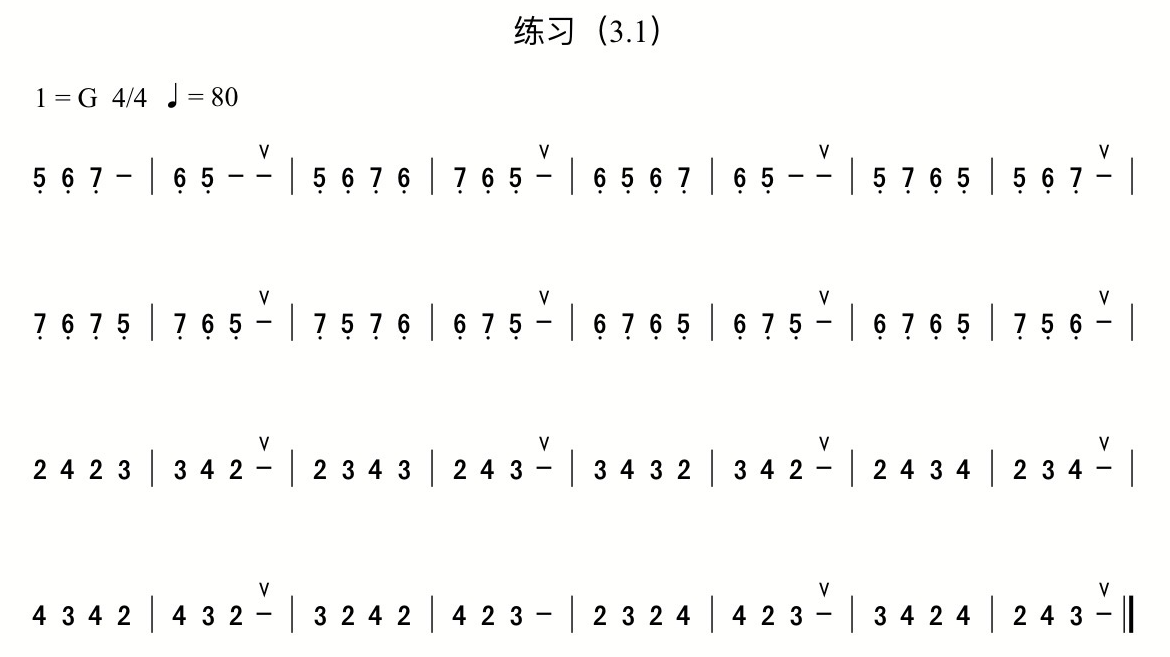
\includegraphics[width=\textwidth]{dongxiao/20200419-练习3.1.png}
	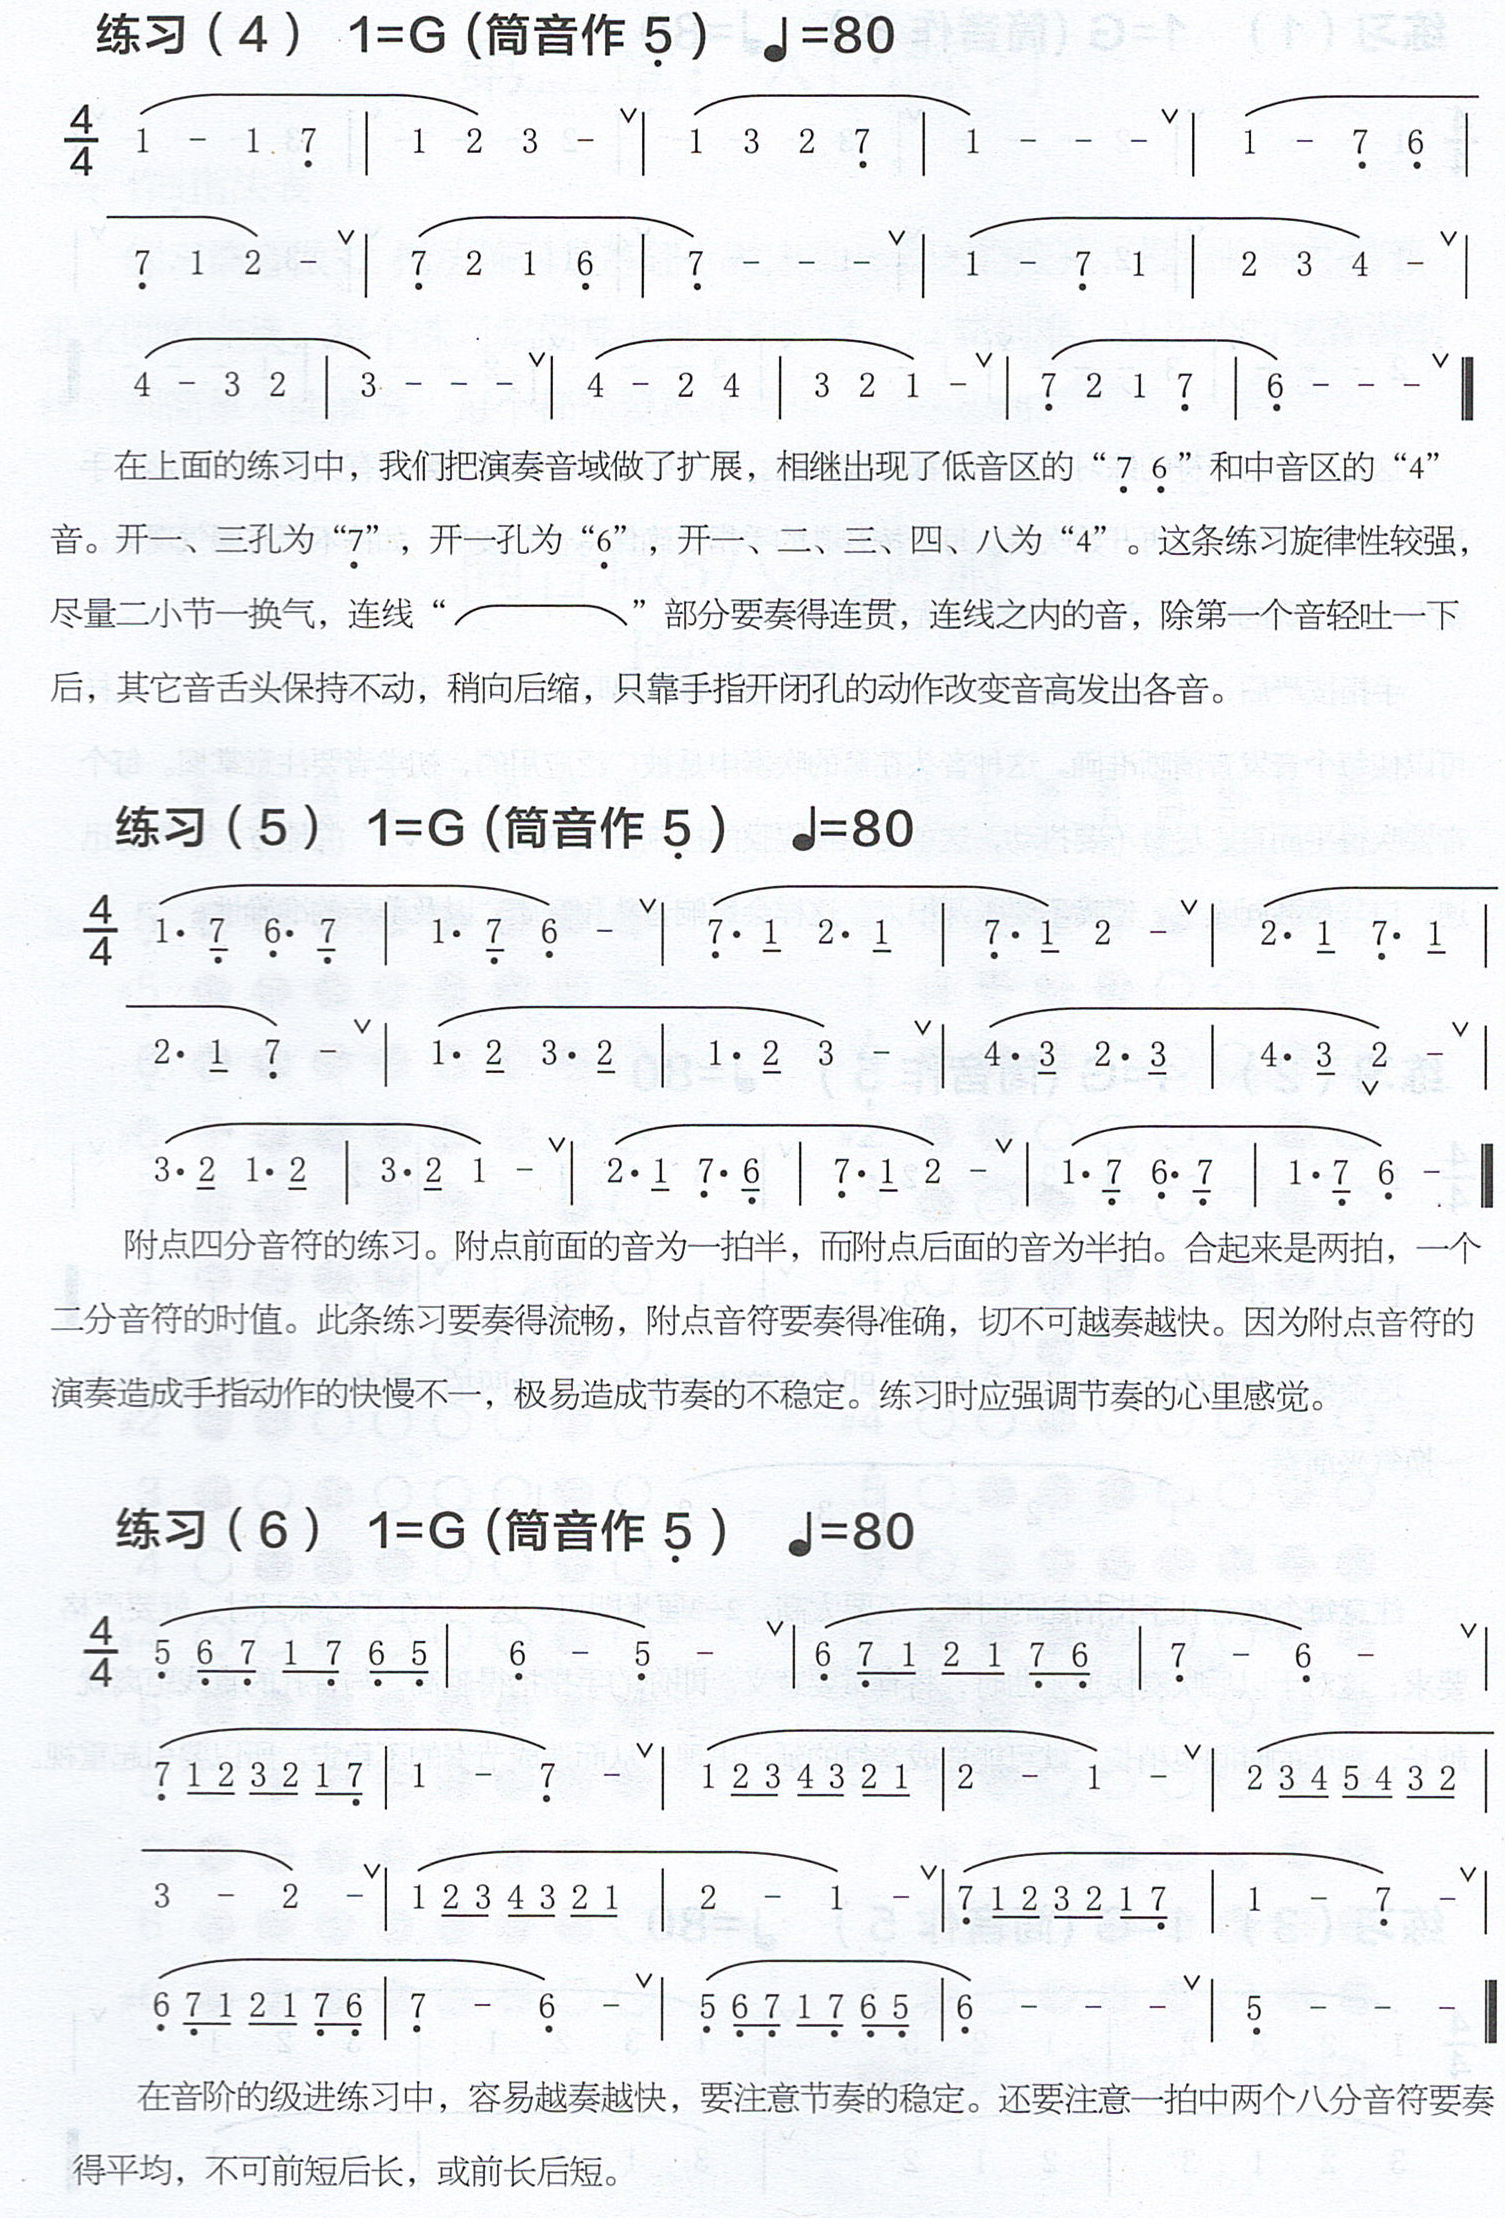
\includegraphics[width=\textwidth]{dongxiao/Scan 2.jpeg}
	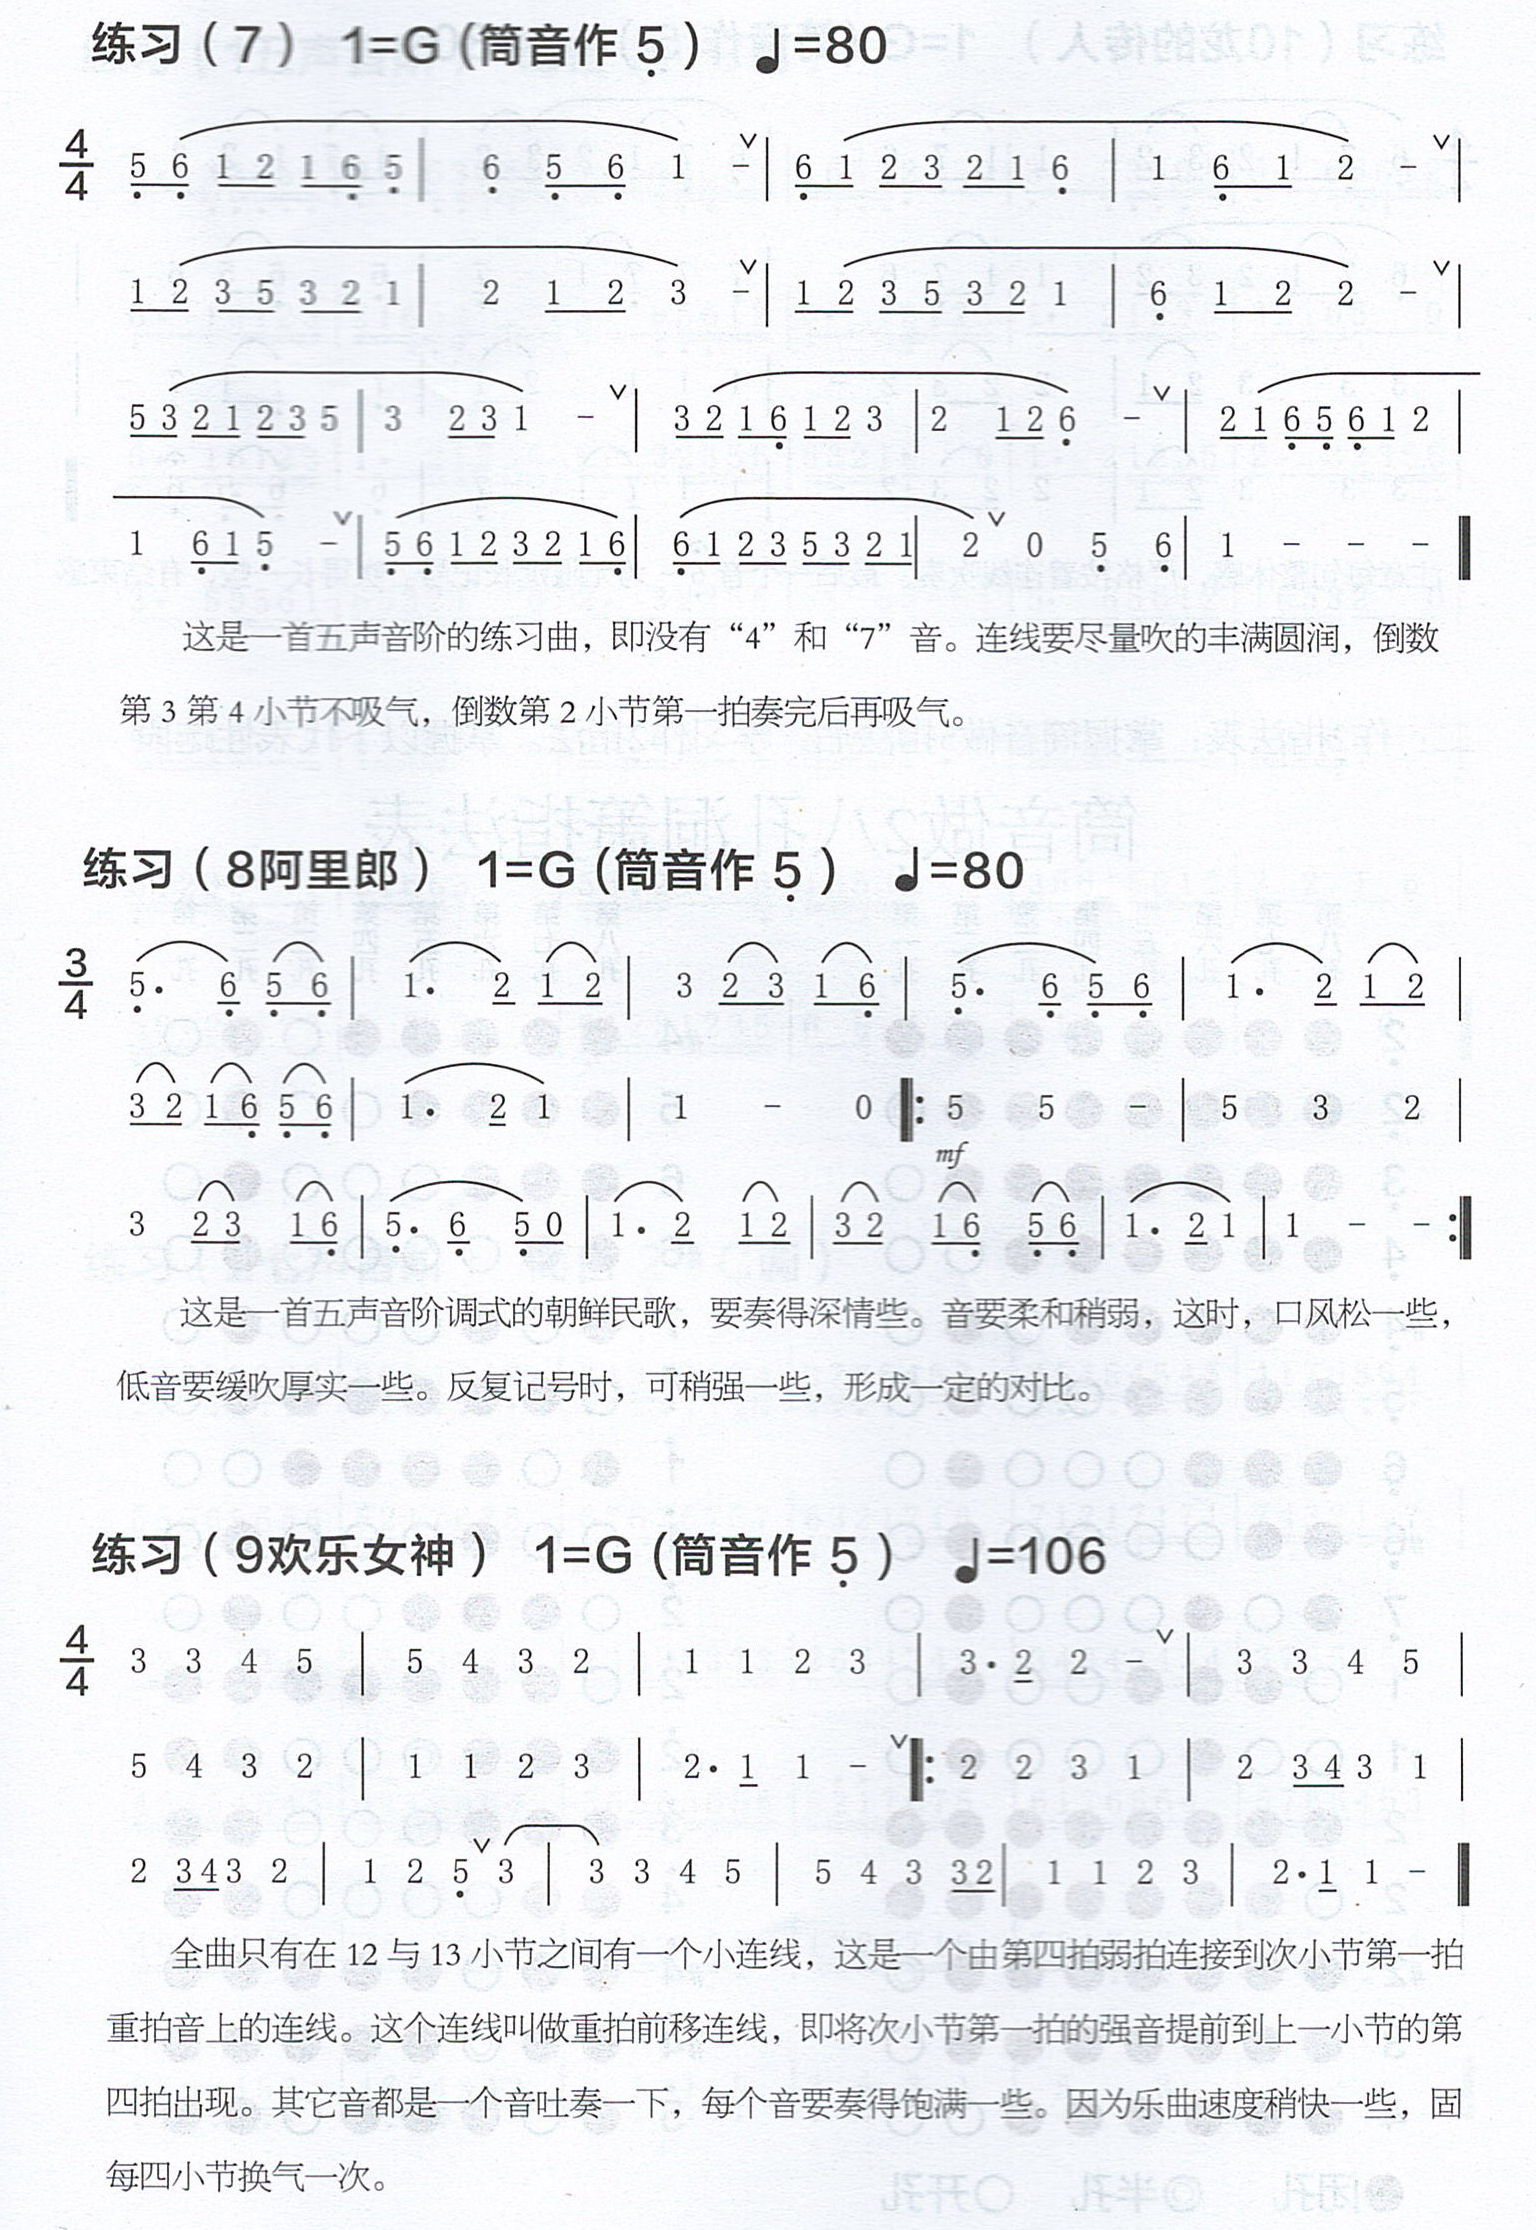
\includegraphics[width=\textwidth]{dongxiao/Scan 3.jpeg}
\end{center}
\chapter{练习谱 - 筒音作2}
	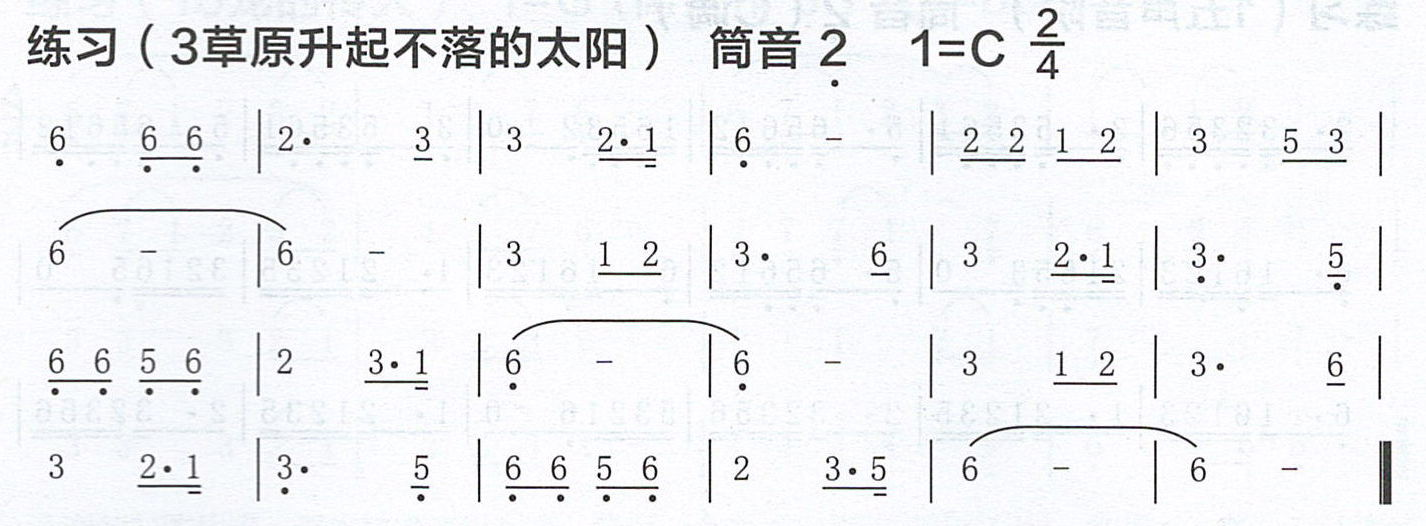
\includegraphics[width=0.8\textwidth]{dongxiao/Scan 6.jpeg}~

\chapter{练习歌曲-首选}
\section{世上只有妈妈好}
	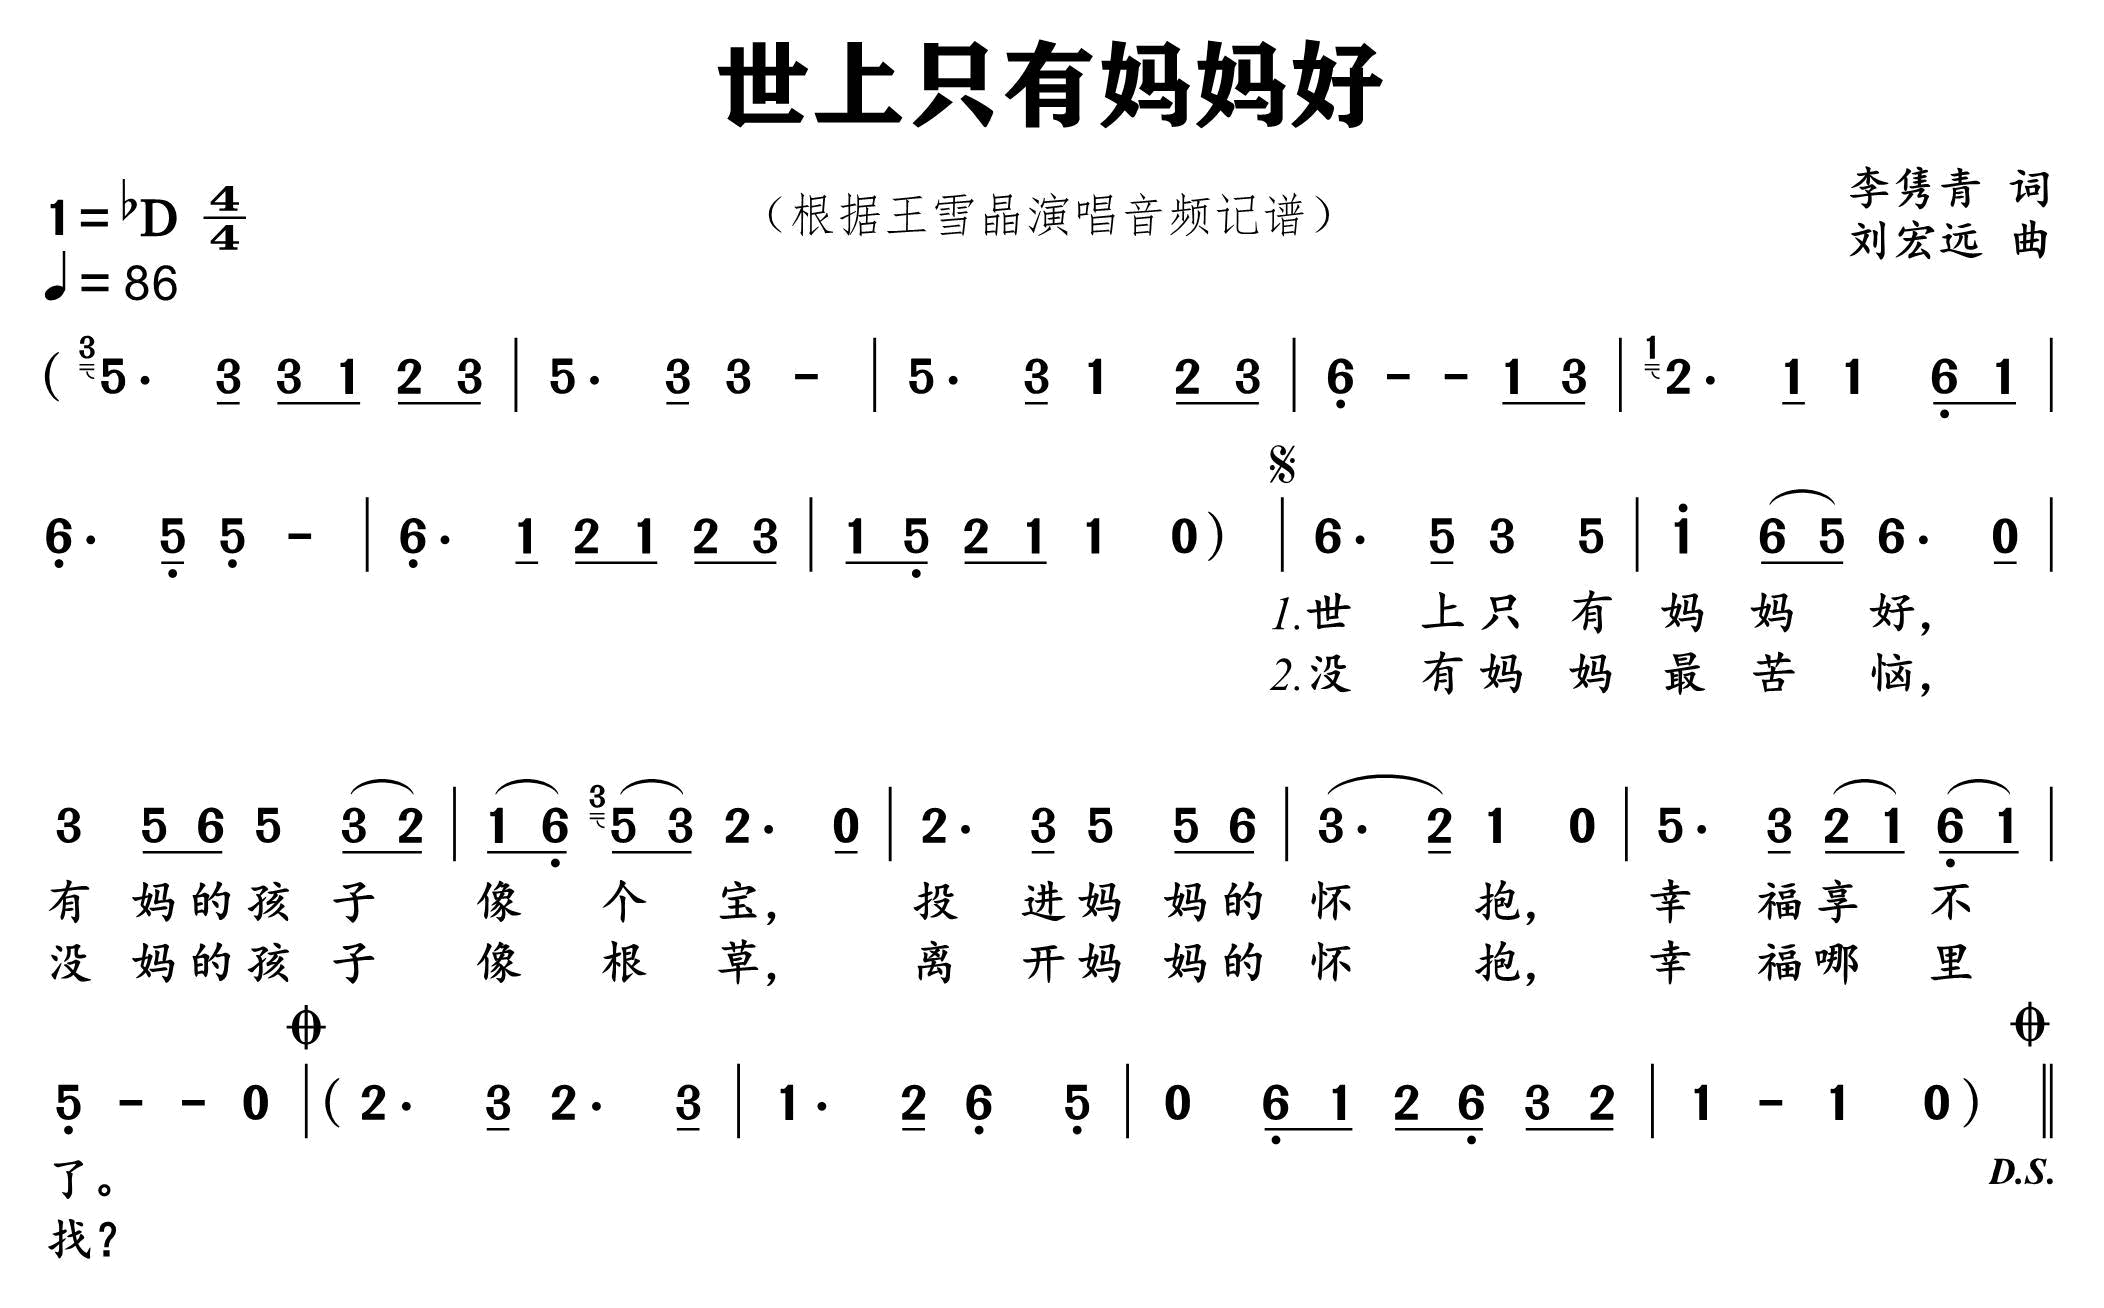
\includegraphics[width=\textwidth]{dongxiao/IMG_0854-世上只有妈妈好.png}
\section{送别}
    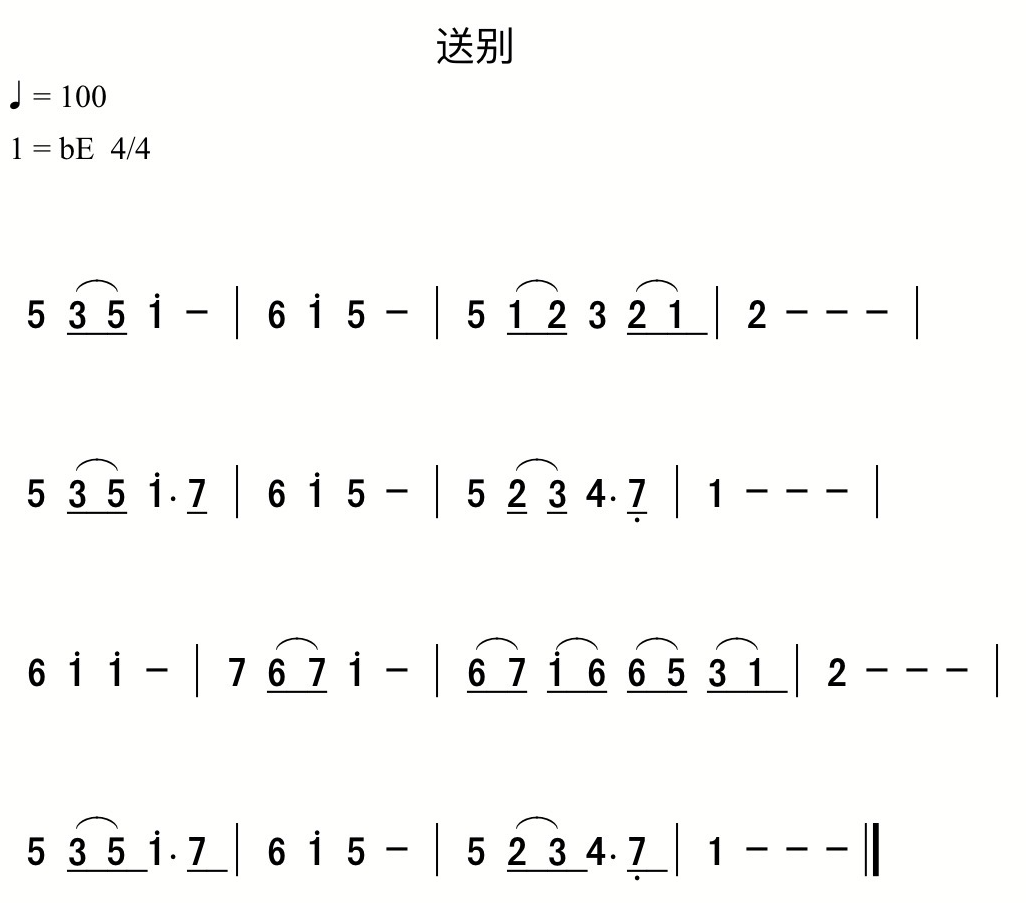
\includegraphics[width=\textwidth]{dongxiao/IMG_0855-送别.png}  
\section{儿女情}          
	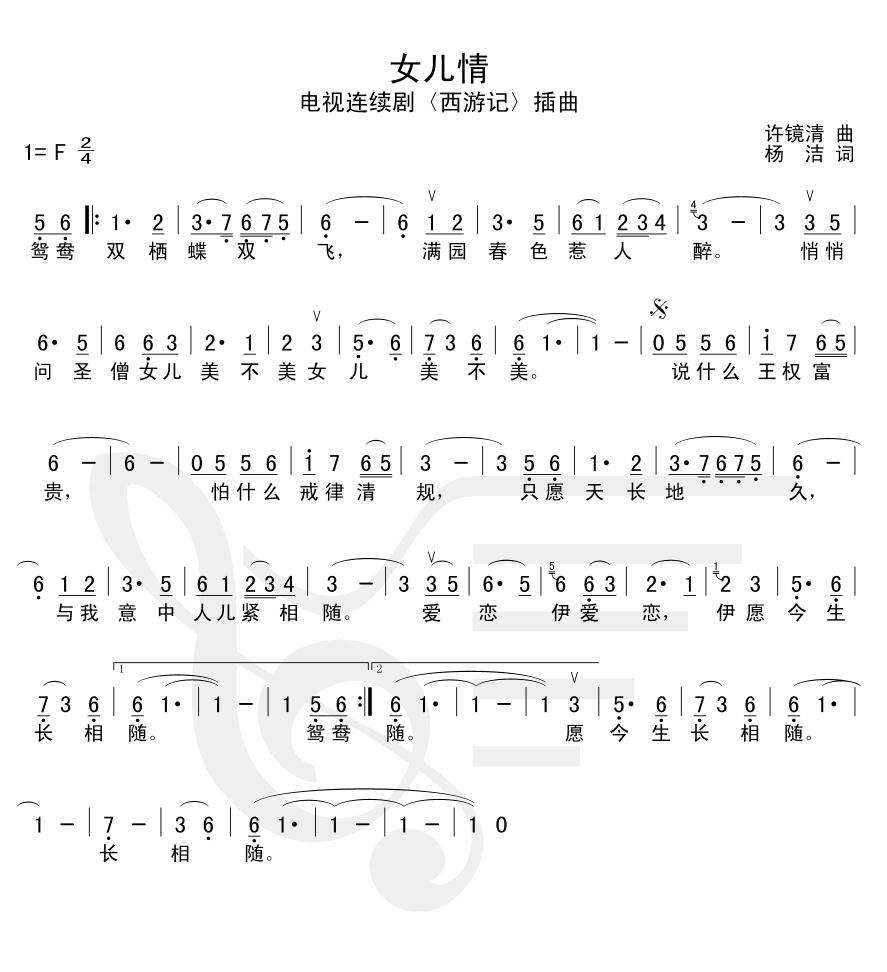
\includegraphics[width=\textwidth]{dongxiao/西游记-儿女情}  
\section{樱花}
	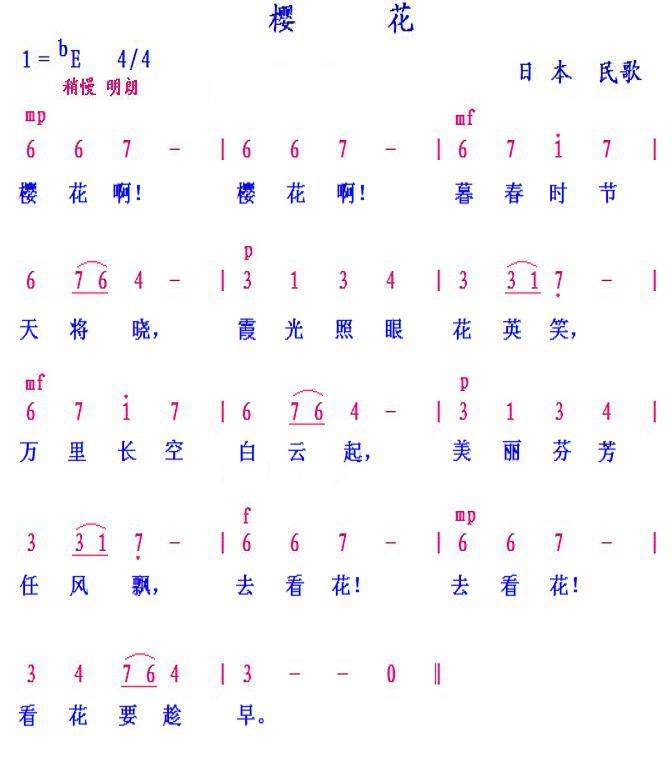
\includegraphics[width=\textwidth]{dongxiao/日本-樱花.jpg}  
\section{时间都去哪儿了}
    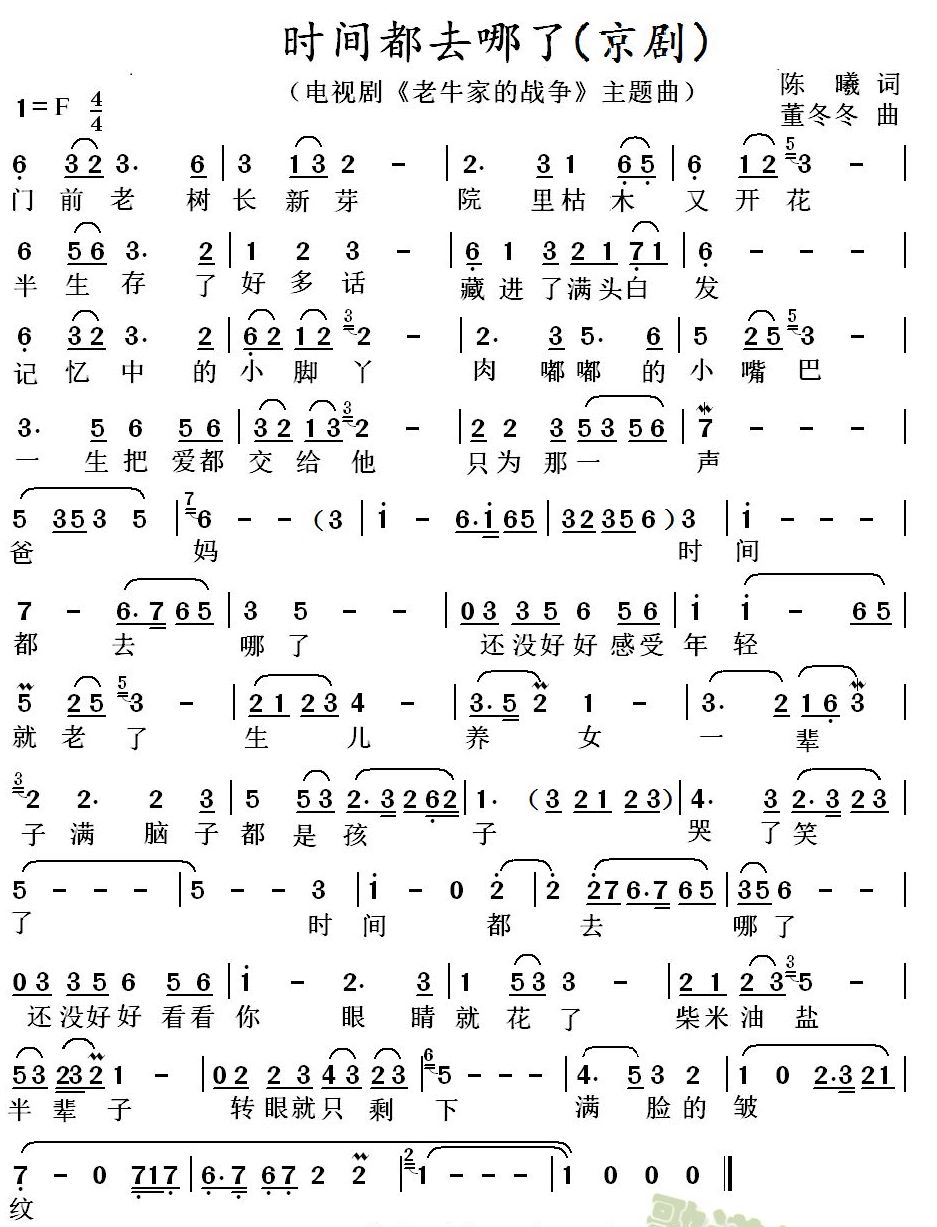
\includegraphics[width=\textwidth]{dongxiao/20200411-时间都去哪儿了.jpg} 
\section{静夜思}
    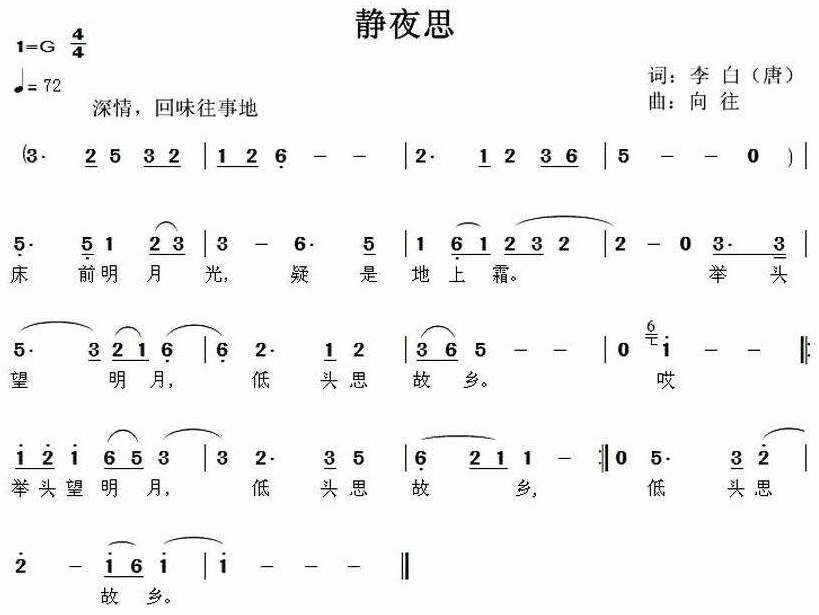
\includegraphics[width=\textwidth]{dongxiao/20200411-静夜思.jpg}
\section{定风波-苏轼词}
    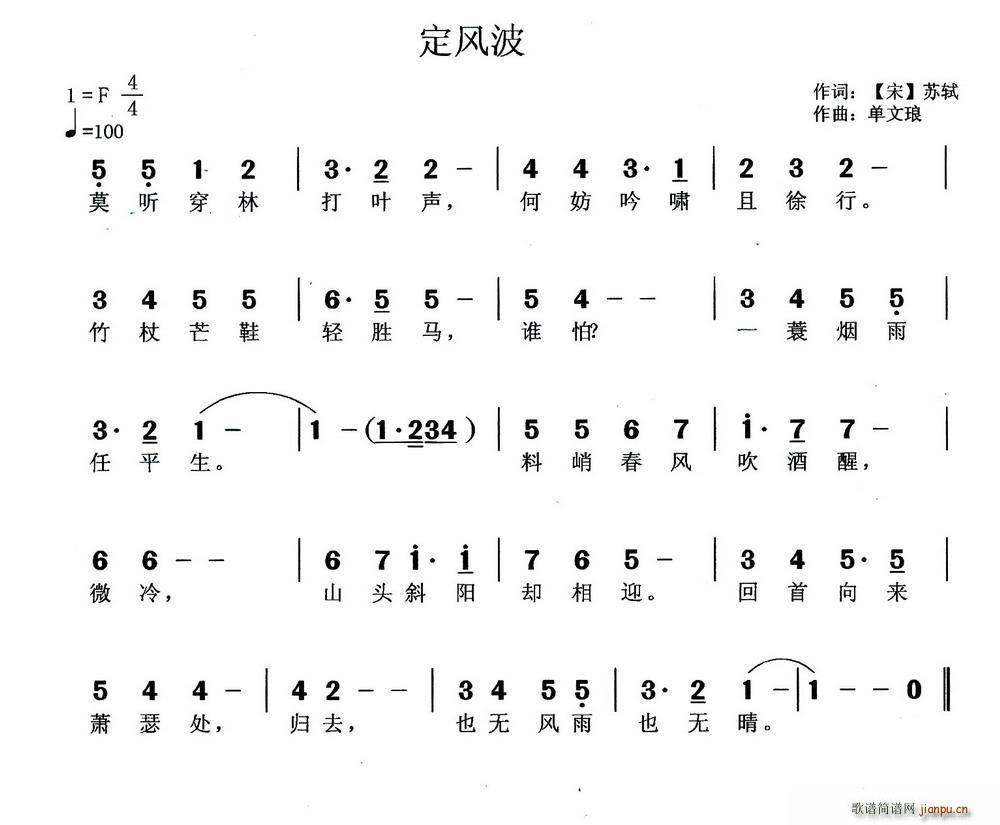
\includegraphics[width=\textwidth]{dongxiao/20200411-定风波.jpg}
\chapter{练习歌曲-曲牌}
\section{关山月}
    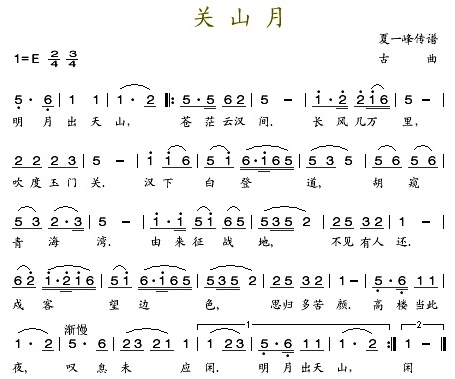
\includegraphics[width=\textwidth]{dongxiao/20200411-清平乐-关山月.jpg}
\section{明月几时有-苏轼词}
    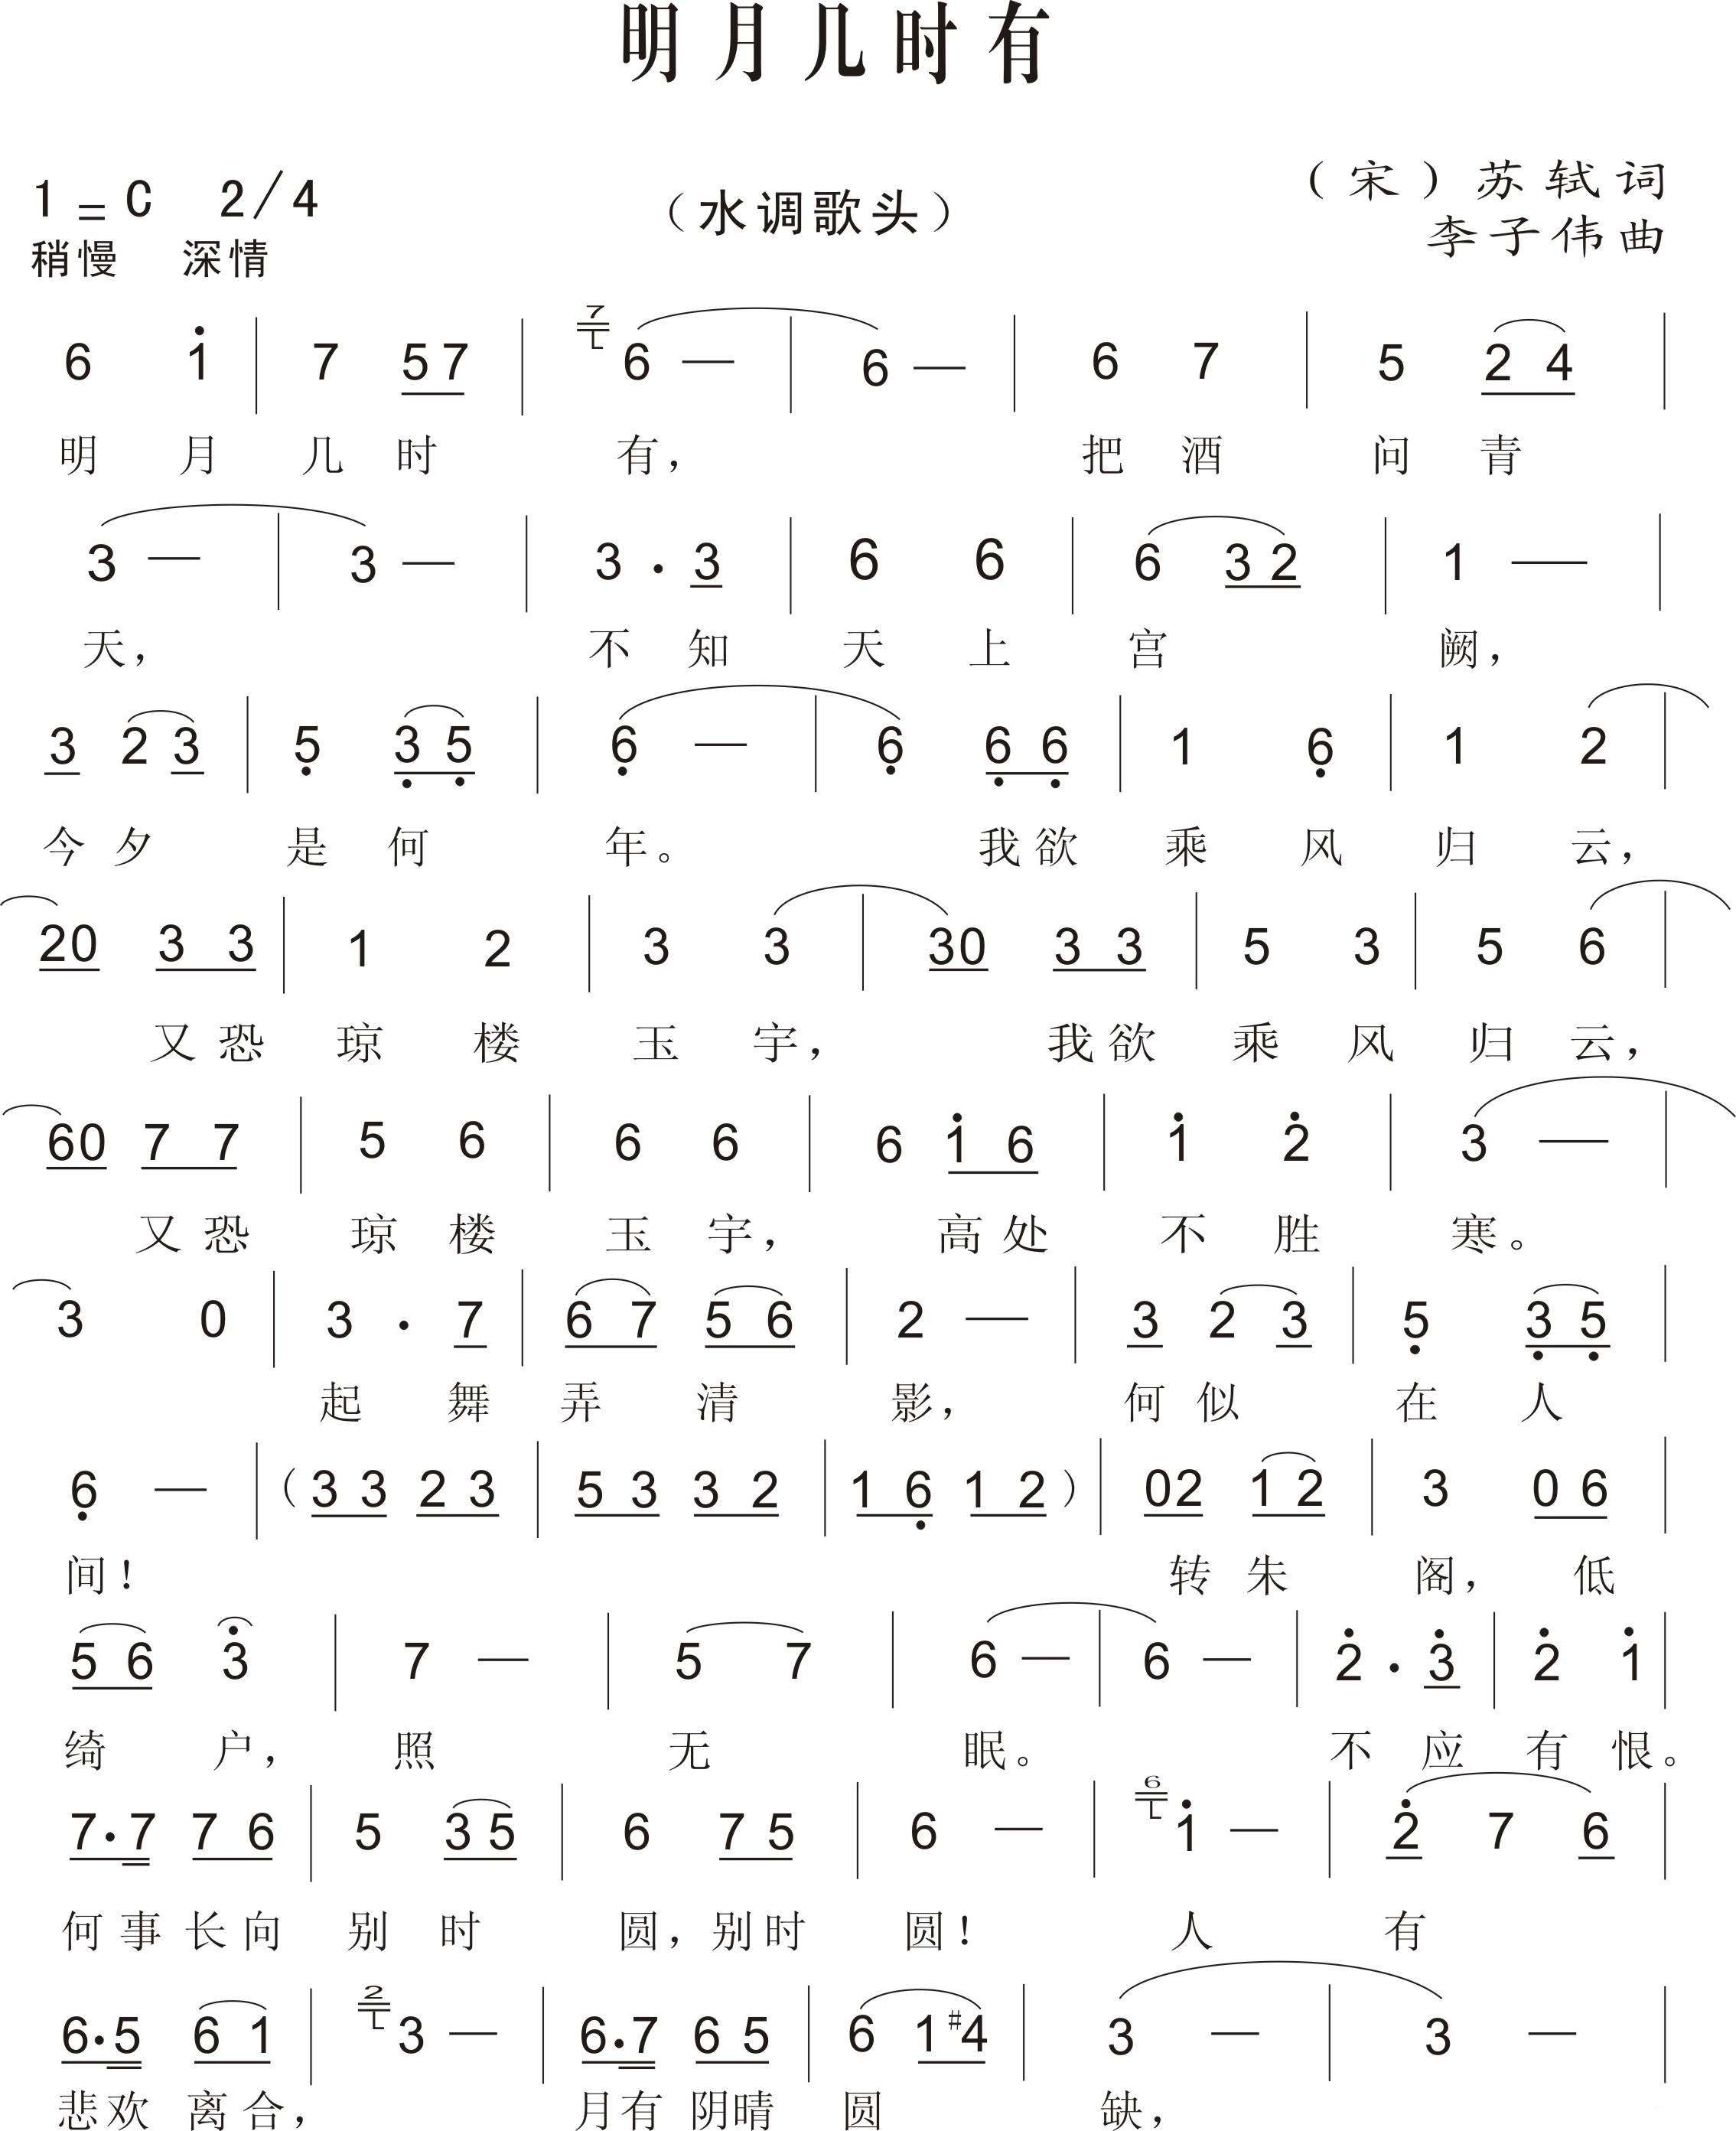
\includegraphics[width=\textwidth]{dongxiao/20200411-明月几时有.jpg}
\section{清平乐-春归何处}
    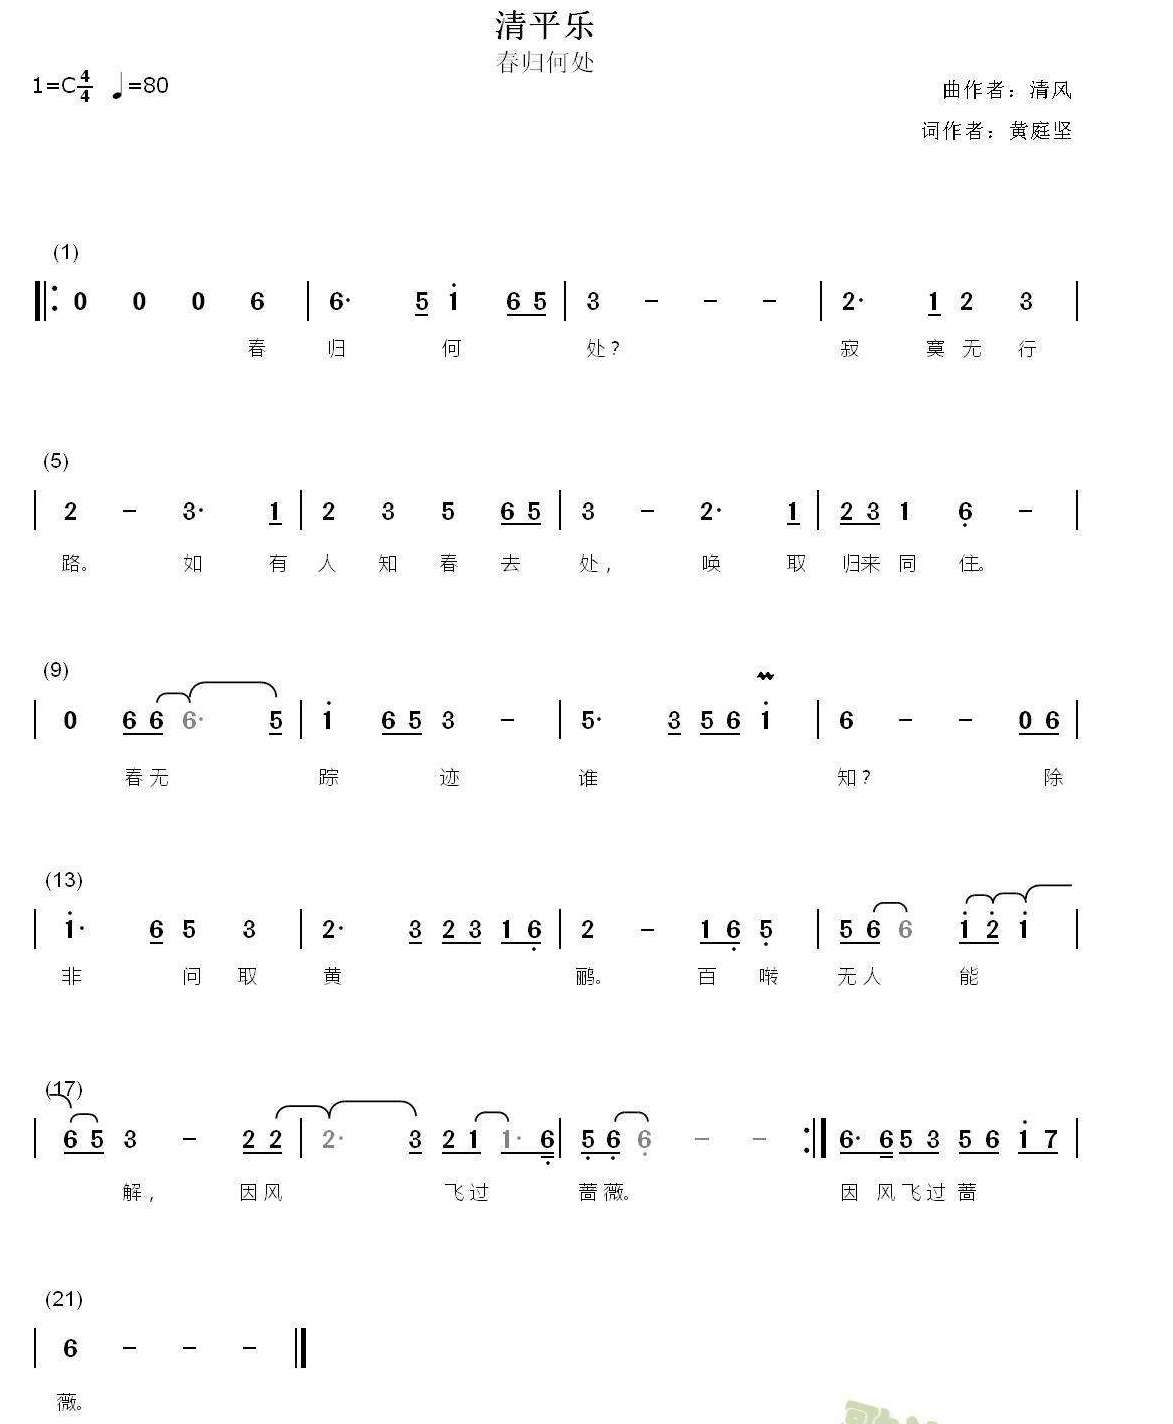
\includegraphics[width=\textwidth]{dongxiao/20200411-清平乐-春归何处.jpg}
\section{清平乐-晏殊词}
    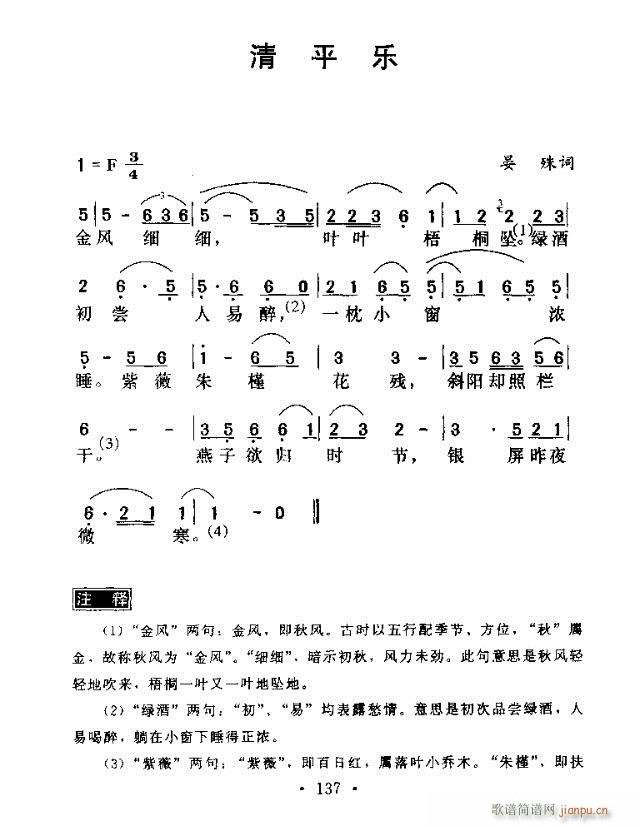
\includegraphics[width=\textwidth]{dongxiao/20200411-清平乐-晏殊.jpg}
\section{蝶恋花-春景}
    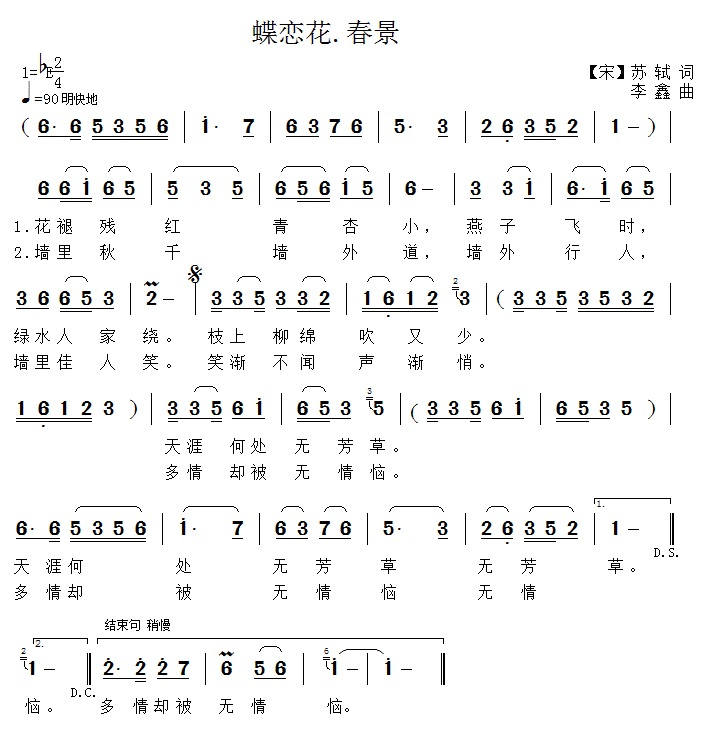
\includegraphics[width=\textwidth]{dongxiao/20200411-蝶恋花-春景.jpg}
\section{城市很静}
    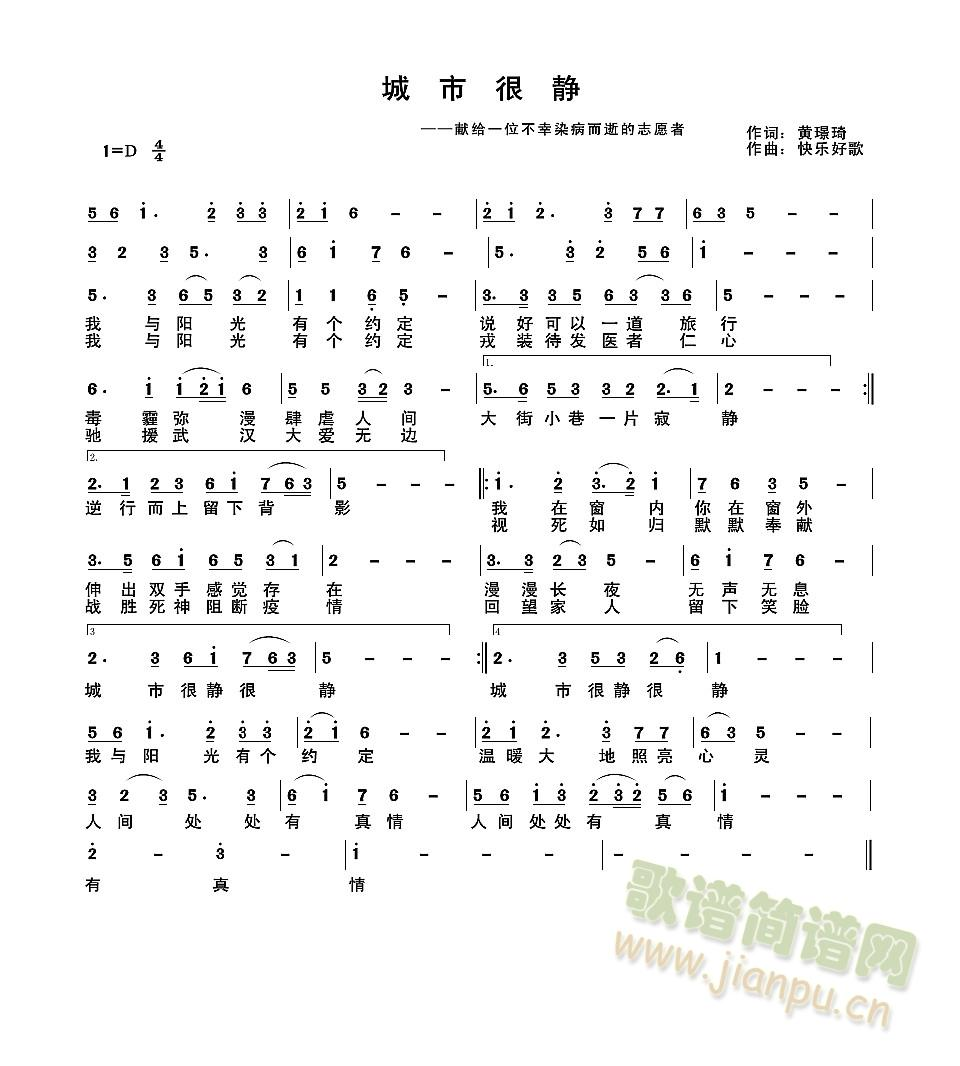
\includegraphics[width=\textwidth]{dongxiao/20200402-城市很静} 
\section{风留念}
    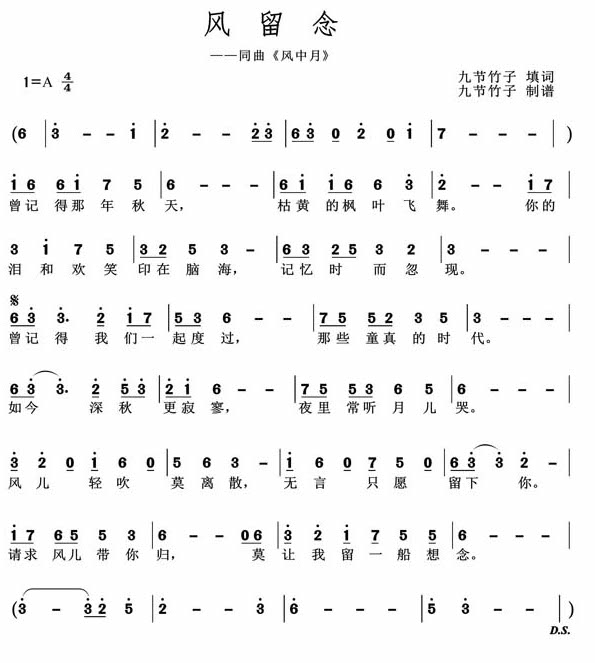
\includegraphics[width=\textwidth]{dongxiao/20200323风留念.jpg}
\section{玉楼春}
    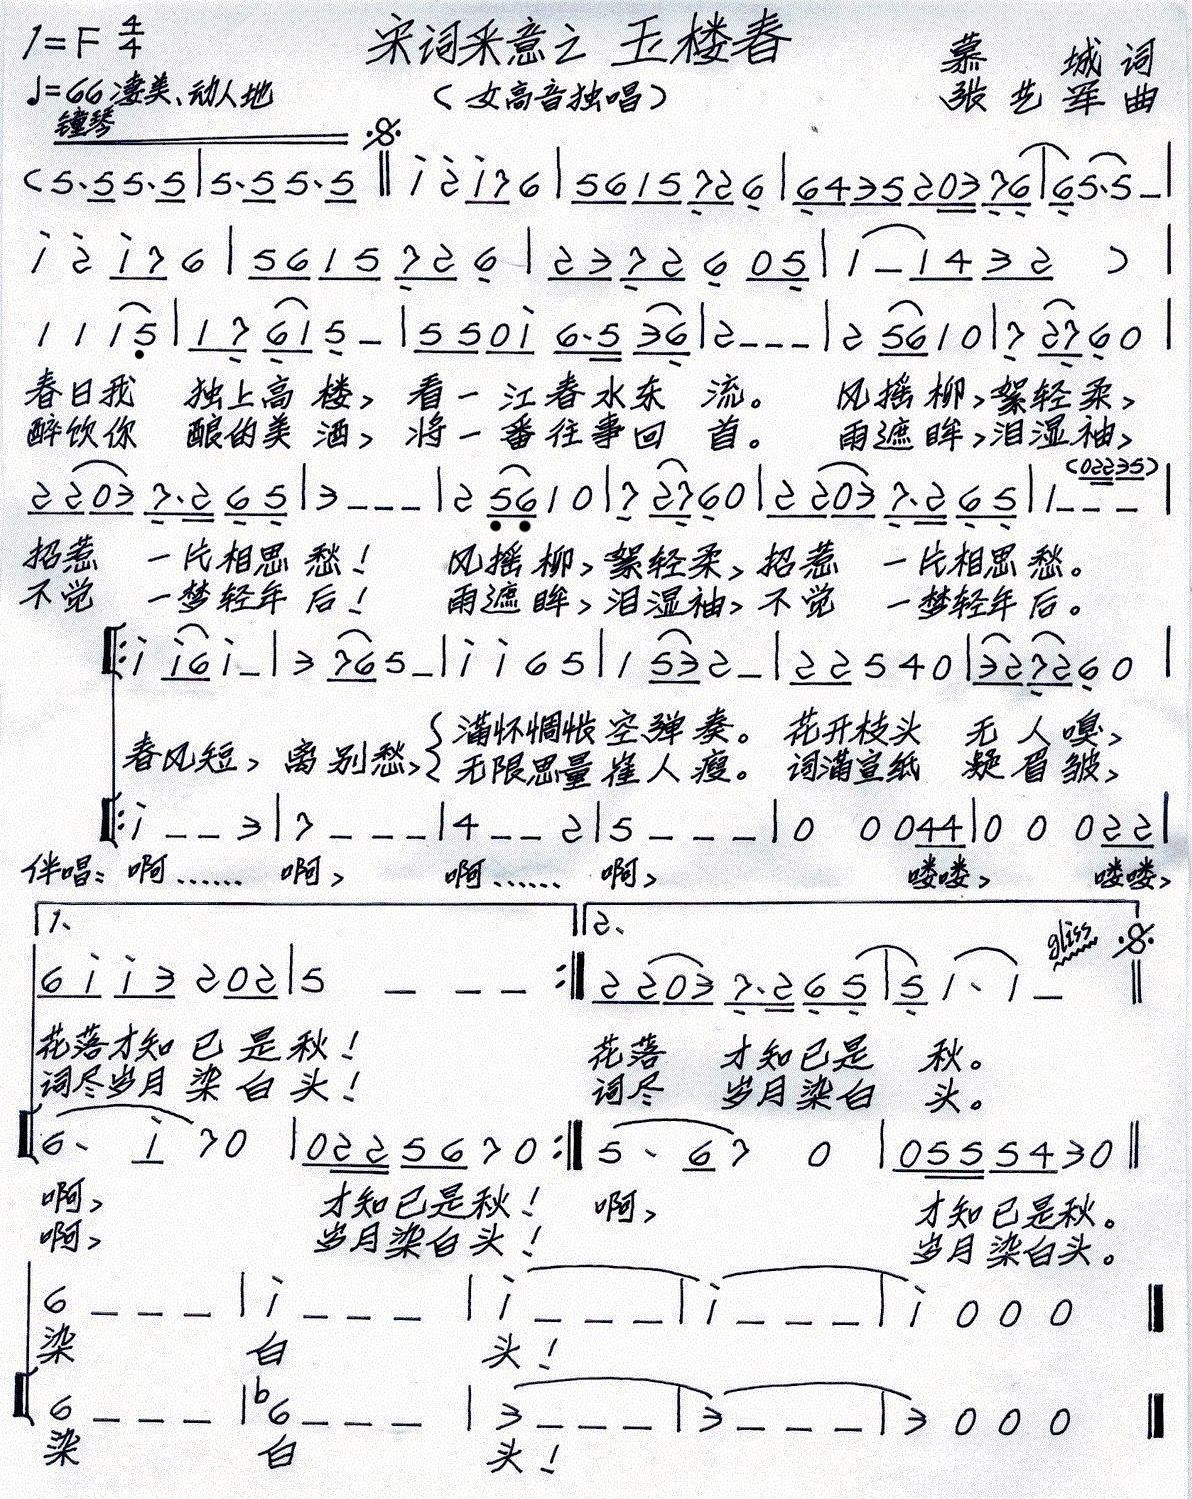
\includegraphics[width=\textwidth]{dongxiao/20200323玉楼春.jpg}
\section{墨香-长安曲}
    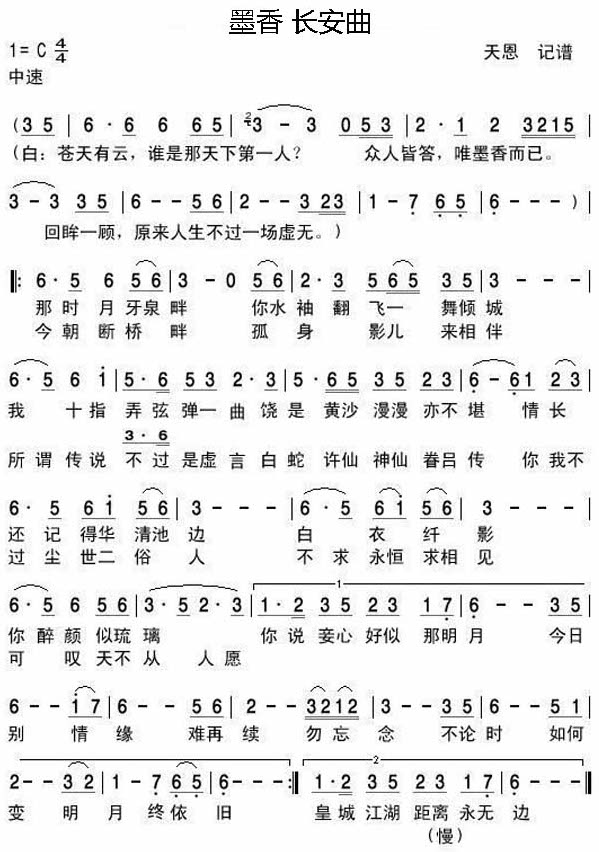
\includegraphics[width=0.9\textwidth]{dongxiao/20200323墨香-长安曲.jpg} 
\section{思美人兮}
    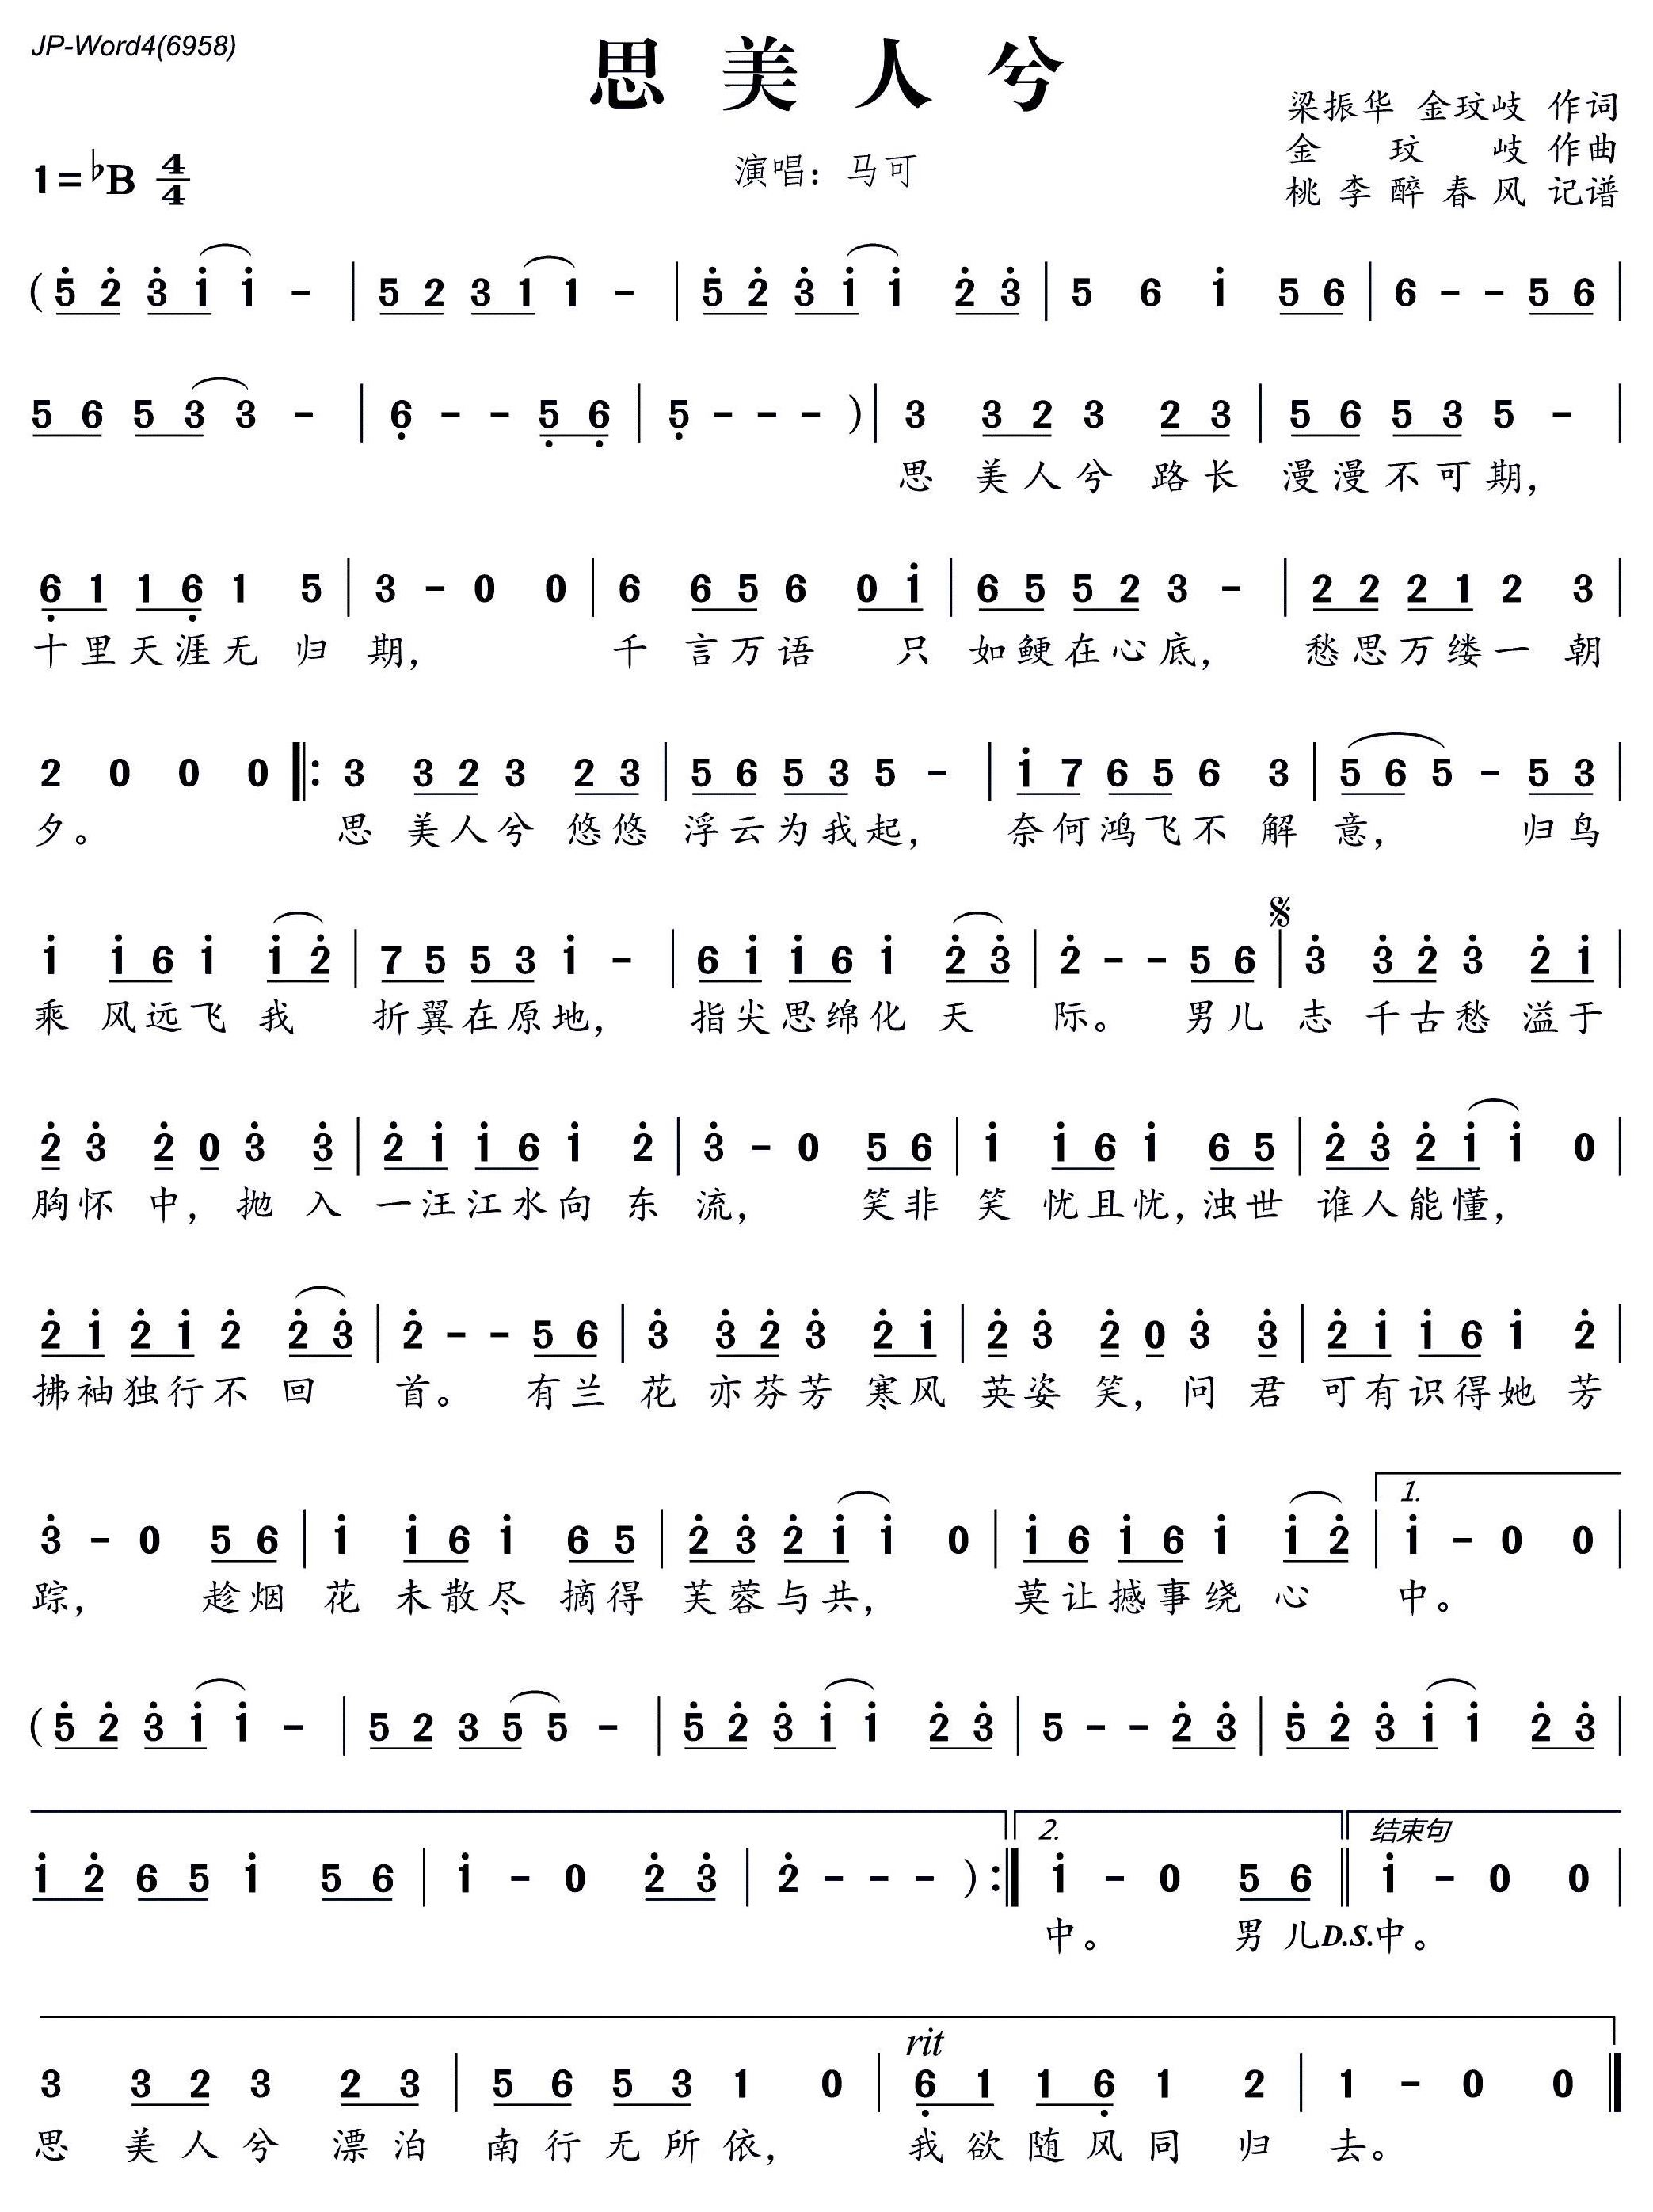
\includegraphics[width=\textwidth]{dongxiao/20200402-思美人.jpg}
\end{document}
